\chapter{Ergebnis und Fazit}\label{ch:fazit}
Ziel des Projekts war die Entwicklung eines modular aufgebauten analogen Synthesizer zur elektronischen Klangsynthese, welches auch erreicht wurde wie in Abbildung \ref{fig:modularer Synthesizer} zu sehen.
Im Zuge des Projekts sollten Fertigkeiten bezüglich Konzeption, Entwurf und Fertigung von analogen Schaltungen erlangt werden.
Es wurde von jedem Teammitglied der komplette Prozess von Konzeption der Schaltung, Simulation der Eigenschaften, Layout einer Leiterplatte und deren Bestückung sowie das Design einer Frontplatte durchlaufen. Somit kann die Weiterentwicklung dieser spezifischen Fertigkeiten als voller Erfolg angesehen werden. Dass grundsätzlich alle Module bis auf einzelne kleine Mängel funktionieren spricht auch für den Erfolg des Projekts.\\
Es konnten bis auf den ADSR und den VCA alle Module realisiert werden. Das liegt an der im Vorfeld etwas unterschätzten Erwartungshaltung bezüglich des Aufwands der tatsächlichen Realisierung inklusive der Bestückung der Leiterplatte, Fehlersuche und Behebung dieser.  
Das ist aber aus Sicht des Teams in Ordnung, da der Großteil der Gruppe noch nie solche Tätigkeiten gemacht hatte.
Neben dem Gewinn an neuen Fertigkeiten war vor allem der Spaß am Entwicklen immer präsent.
Abschließend bedanken wir uns bei Herrn Zimmermann für das schnelle und zuverlässige Abwickeln der Bauteil-Bestellungen und die Betreuung im Labor und bei Herrn von Hoffmann für die gute Zusammenarbeit.


\begin{figure}[h]
	\centering
	\setlength{\fboxsep}{1pt} %Abstand der Linien zur Abbildung
	\setlength{\fboxrule}{1pt} %Dicke der Linie
	\fbox{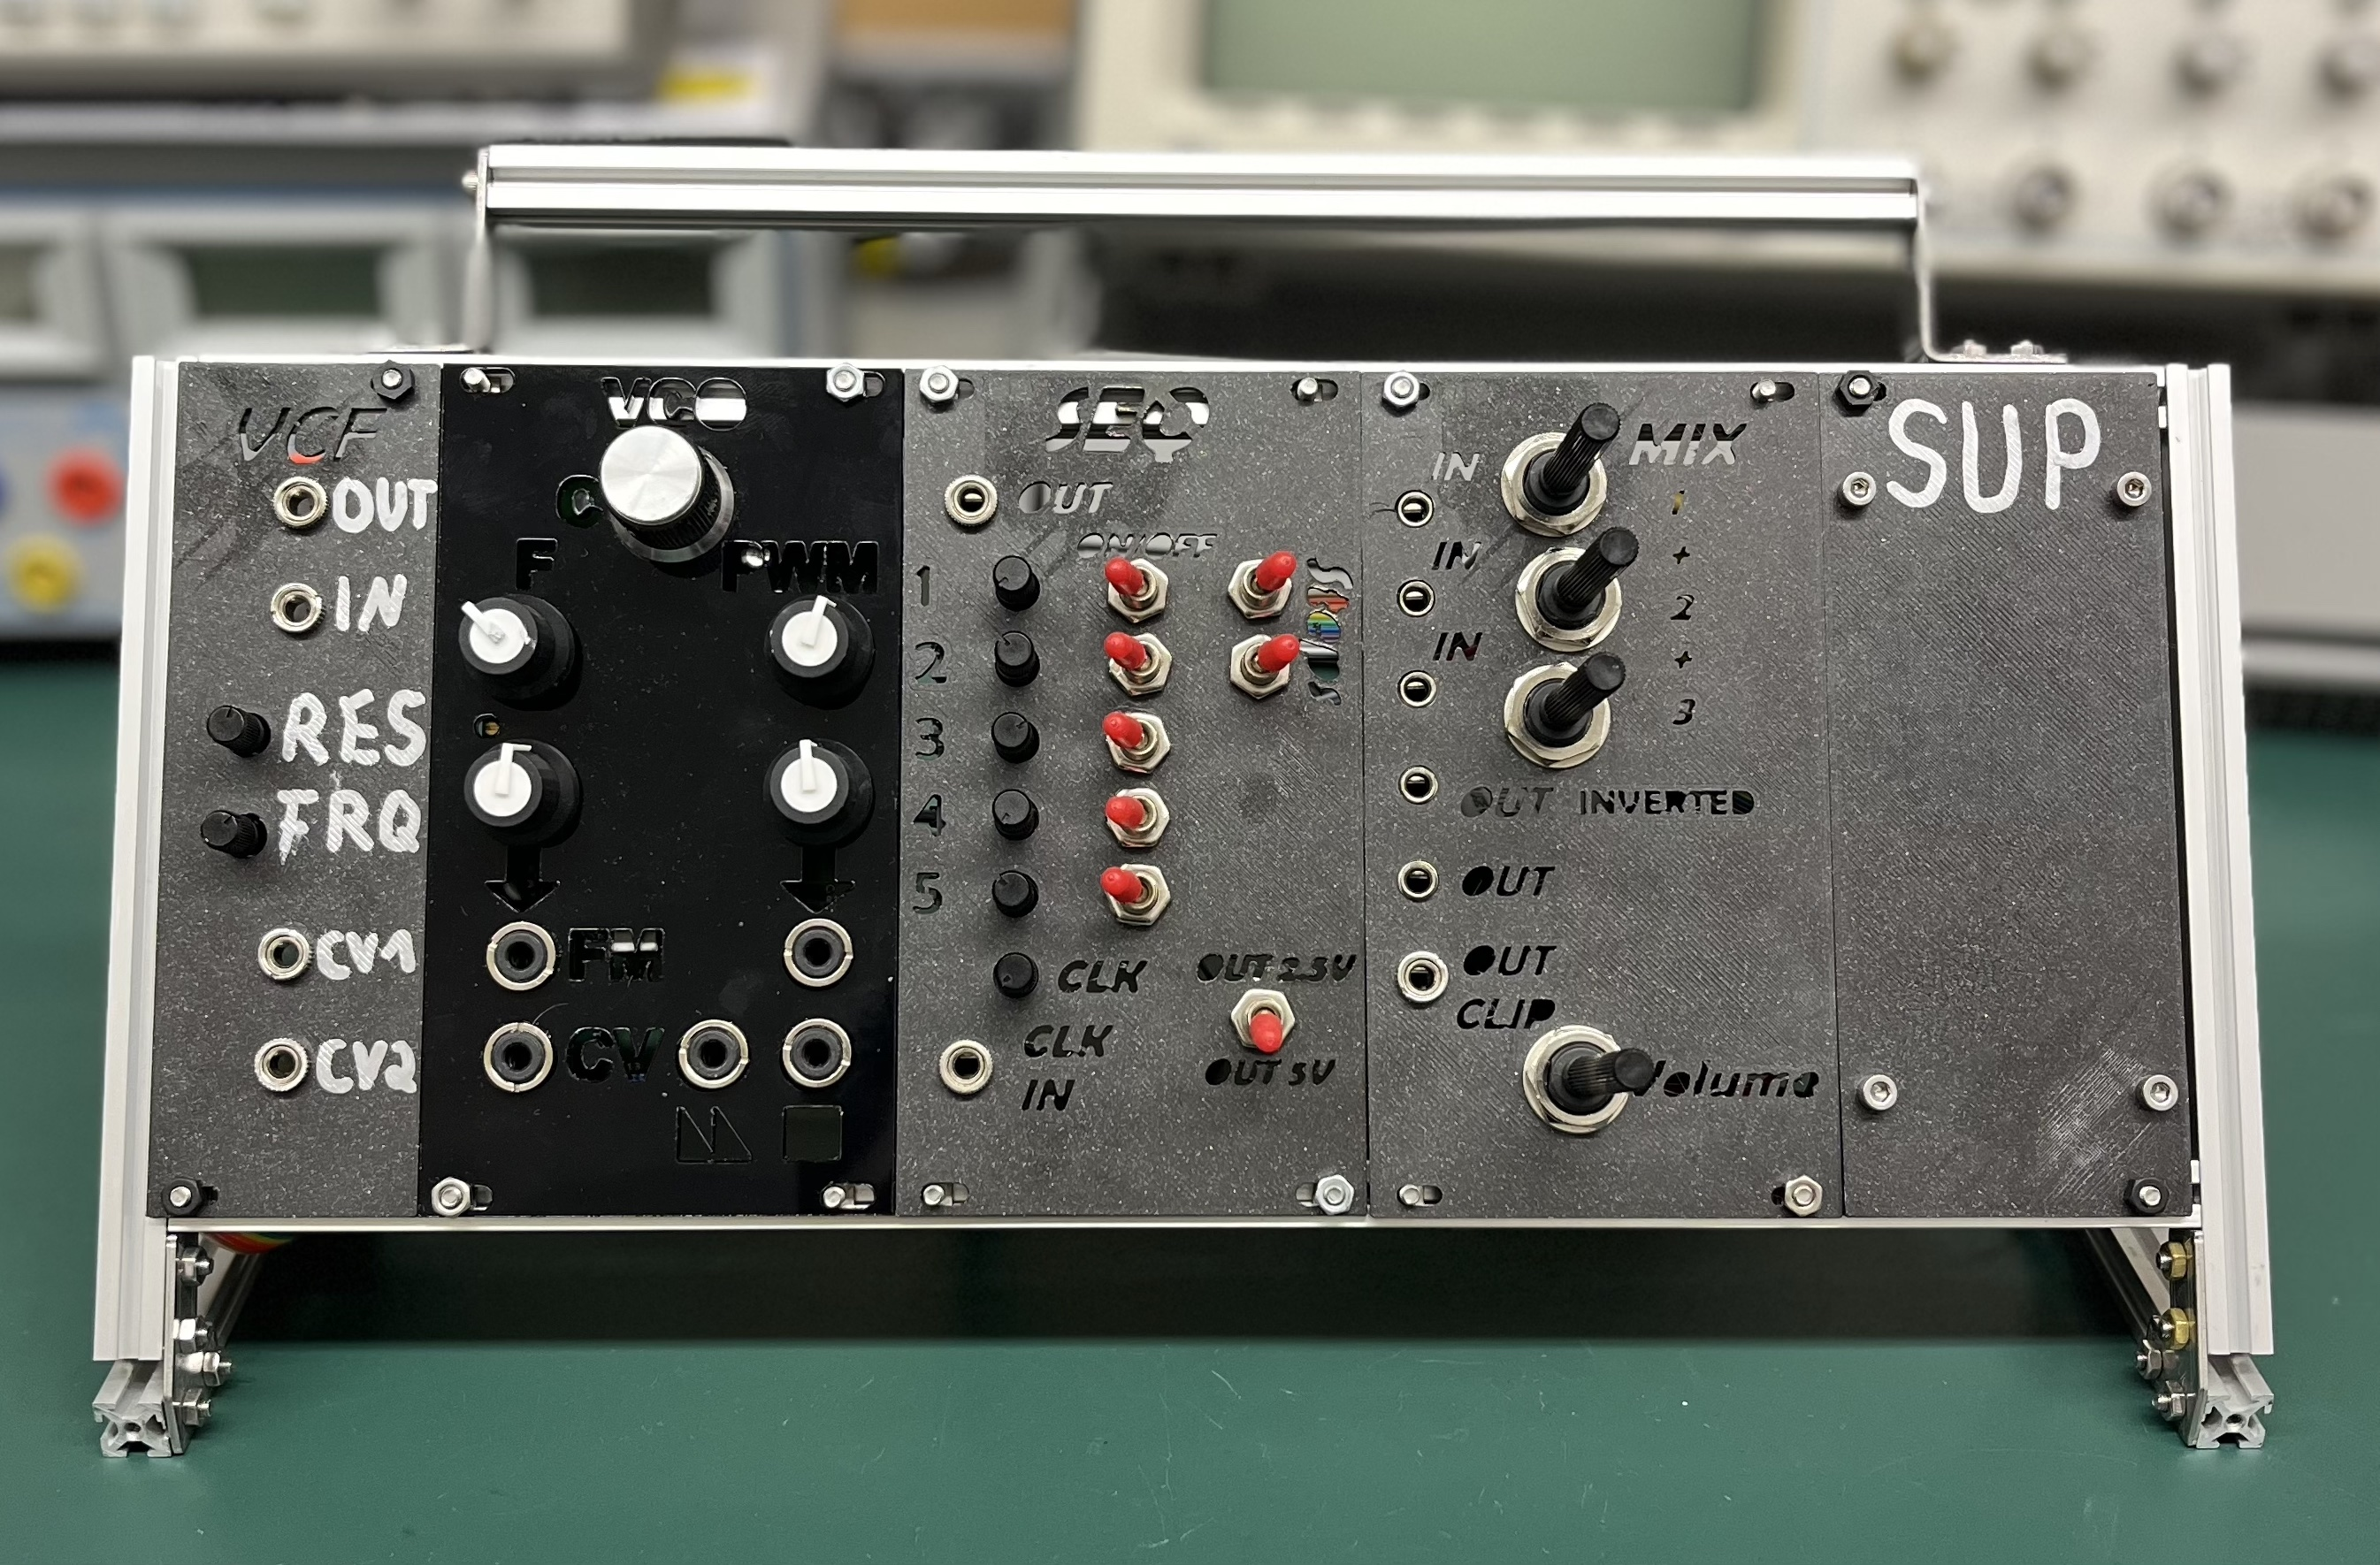
\includegraphics[width=0.8\textwidth]{figures/Synthesizer_Rack}}
	\caption{modularer Synthesizer}
	\label{fig:modularer Synthesizer}
\end{figure}

